\newpage
\begin{center}
	\textbf{\large ГЛАВА 4 \\ МОДЕЛИРОВАНИЕ И СБОРКА}
\end{center}
\refstepcounter{chapter}


% \section*{}
\addcontentsline{toc}{chapter}{ГЛАВА 4}
\section{Общие требования к физической модели четырехногого робота.}\label{C4_1}

Все четвероногие животные при движении сохраняют равновесие почти исключительно за счет динамической устойчивости. Изначально план чередования опорных и свободных положений ног заключался в переключении фаз по принципу ноги 1-4 опорная фаза, ноги 2-3 свободная, как показано на рисунке \ref{cycle_wanted}. Зелеными стрелками обозначены фазы свободного положения, а красными опорного. Однако, такой подход не совсем точен, хоть и вполне логичен.
\begin{figure}[h!]
	\begin{center}
		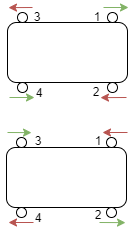
\includegraphics[width=0.3\textwidth]{cycle_wanted}
		\caption{Смена опорных и свободных фаз.}
		\label{cycle_wanted}
	\end{center}
\end{figure}

  В случае искусственных шагающих аппаратов походка должны быть определена таким образом, чтобы центр тяжести аппарата постоянно находился внутри треугольника, вершинами которого являются конечности, находящиеся на данный момент времени в опорном положении (рисунок \ref{diagrama}). На практике эта возможность была реализована д-ром Такути из Научно-исследовательского центра проблем механики. Под его руководством был разработан шагающий аппарат с четырьмя конечностями, у которых скорость движения в фазе восстановления подобрана так, что длительность этой фазы втрое меньше длительности каждой рабочей фазы. В результате в данный момент времени лишь одна нога робота находится в воздухе, а корпус опирается на три остальные, сохраняя тем самым статическую устойчивость. 
  
  Показанные на рисунке заштрихованные треугольники (так называемые опорные треугольники) образованы вершинами, которые соответствуют текущим точкам касания опорной поверхности какими-либо тремя из четырех ног робота. Например, в состоянии, соответствующем рисунку \ref{diagrama}, опоры касаются три ноги - А, В, С, а четвертая нога - D, будучи в фазе восстановления, находится в воздухе. Для обеспечения статической устойчивости принципиально важное значение имеет правильный выбор порядка чередования (сдвиг фаз) четырех ног в процессе движения аппарата. В момент времени, отраженный на диаграмме 1, нога В только что коснулась земли и сейчас занимает опорное положение, нога А также касается земли, но находится уже во второй половине своей рабочей фазы, а нога С - еще в первой половине собственной рабочей фазы. Нога D, находящаяся в момент наблюдения в воздухе, быстро заканчивает фазу восстановления, и к моменту времени, которому соответствует диаграмма 2, она уже опускается на землю, переходя в опорное положение. К этому моменту нога А завершила свою рабочую фазу и, оторвавшись от земли, переходит в фазу восстановления; нога В находится в первой половине, а нога С - во второй половине своих рабочих фаз. Аналогично в следующие моменты времени, которым соответствуют диаграммы 3 и 4, в фазу восстановления переходят друг за другом нога С и нога В. 
  
  При таком порядке чередования ног в любой момент времени, когда одна из ног робота находится в фазе восстановления, центр тяжести аппарата обязательно будет лежать внутри треугольника, образованного тремя ногами, находящимися не в рабочей фазе (опирающимися на землю).
  
\begin{figure}[h!]
  	\begin{center}
  		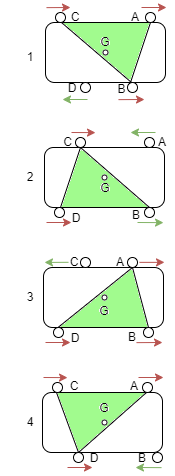
\includegraphics[width=0.5\textwidth]{diagrama}
  		\caption{Смена опорных и свободных фаз с учетом тяжести.}
  		\label{diagrama}
  	\end{center}
\end{figure}

\newpage

\section{Проектирование ног.}\label{C4_2}

В разделе \ref{C1_2} были представлены особенности конструкции и основные проблемы, которые необходимо решить перед производством деталей. 

Для минимизации проблем, связанных с соосностью отверстий, отношениями и масштабами между конструкциями перед этапом печати, были использовали трехмерные твердотельные чертежи при проектировании ног в формате 3D (рисунок \ref{leg_3D}). В качестве материала для изготовления деталей ног был выбран пластик, который используется при печати с помощью 3D-принтера, поскольку уникальная конструкция ног не позволяет использовать доступные металлические изделия для сборки. Кроме того, использование пластика значительно снижает вес конструкции, что позволяет использовать менее мощные двигатели для создания прототипа. Напечатанные и собранные конструкции ног отображены на рисунках \ref{leg2}, \ref{leg3}.  
\begin{figure}[h!]
	\begin{center}
		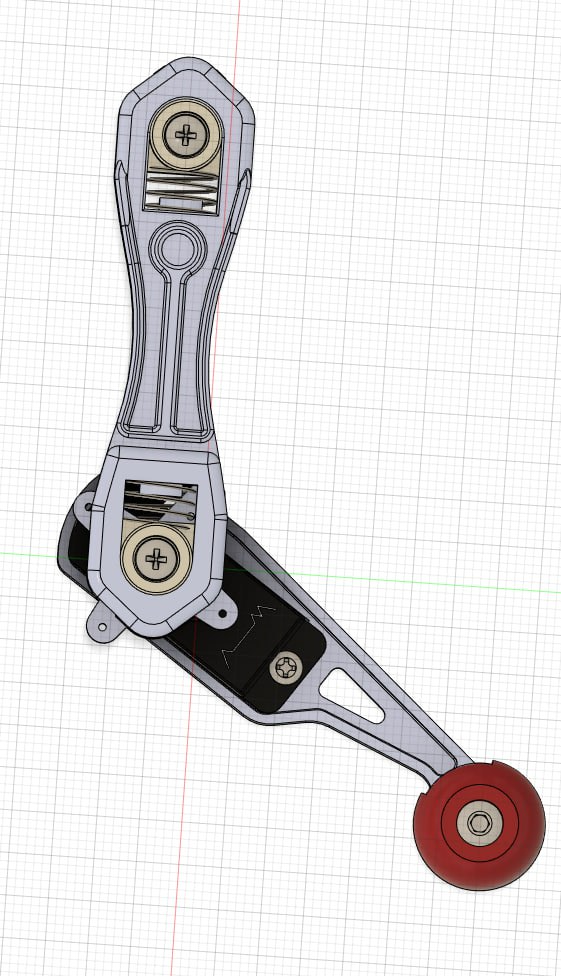
\includegraphics[width=0.45\textwidth]{leg_3D}
		\caption{Твердотельный чертеж ноги робота.}
		\label{leg_3D}
	\end{center}
\end{figure}

\newpage
Сервоприводы, как в сочленении ног, так и в месте соединения с корпусом, закреплены к ползуну, который в свою очередь подпирается пружиной. Ползун обладает "Т" \space образной формой (рисунок \ref{polzun}), которая поддерживает его в плоскости ноги и не дает покинуть область конструкции. 

Пружина служит в качестве демпфера, который гасит ударные воздействия на вал двигателя при движении робота, а также оказывает некоторое полезное сопротивление при резком изменении угла поворота двигателя, что не раз спасало прототип при "живом" \space тестировании походки.

\begin{figure}[h!]
	\begin{center}
		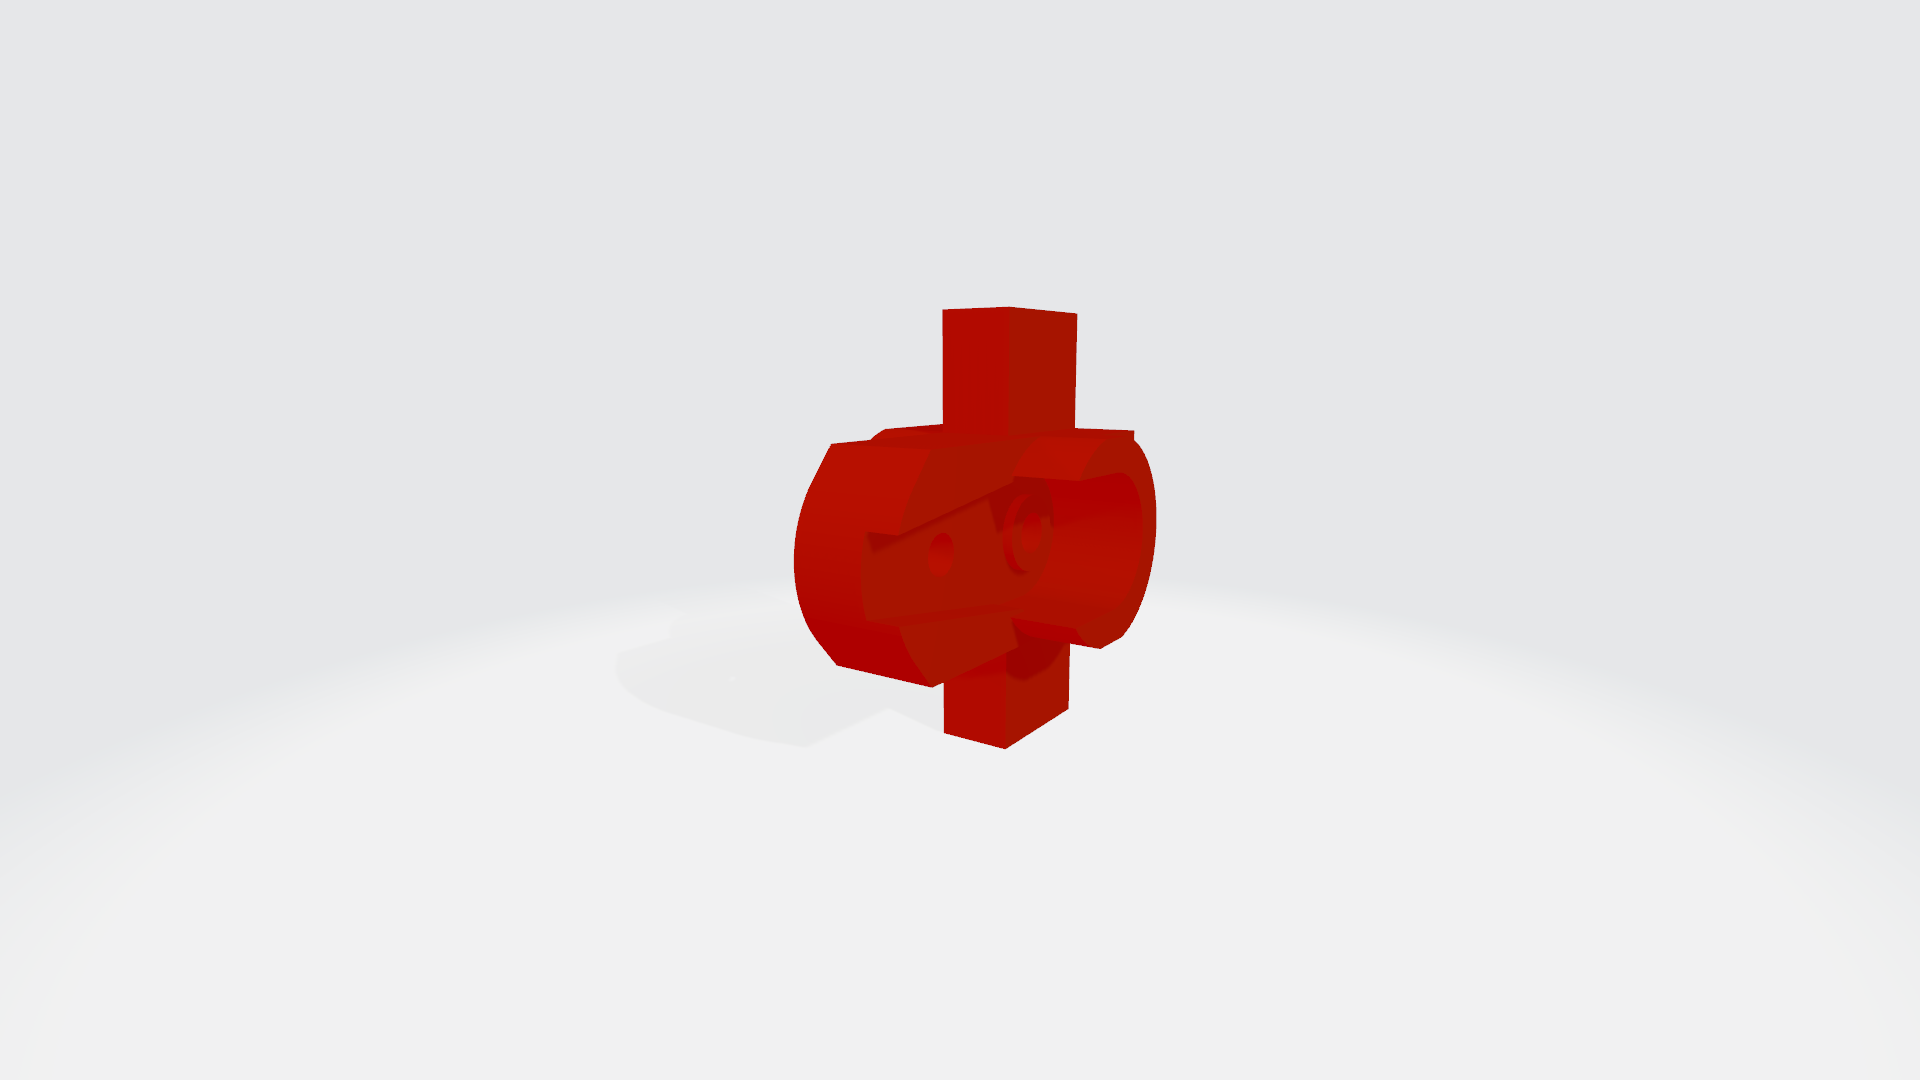
\includegraphics[width=0.6\textwidth]{polzun}
		\caption{\text{''T''} - образный ползун.}
		\label{polzun}
	\end{center}
\end{figure}
\newpage
\begin{figure}[h!]
	\begin{center}
		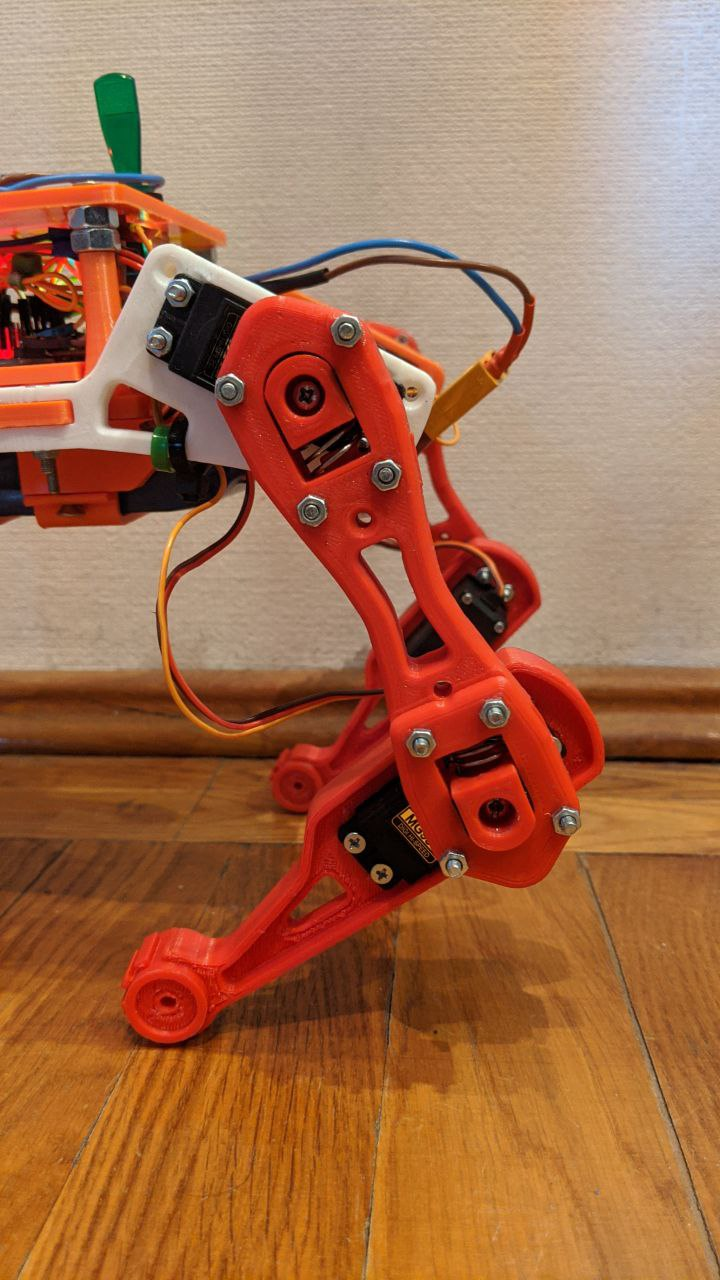
\includegraphics[width=0.4\textwidth]{leg2}
		\caption{Напечатанная нога в сборке.}
		\label{leg2}
	\end{center}
\end{figure}

\begin{figure}[h!]
	\begin{center}
		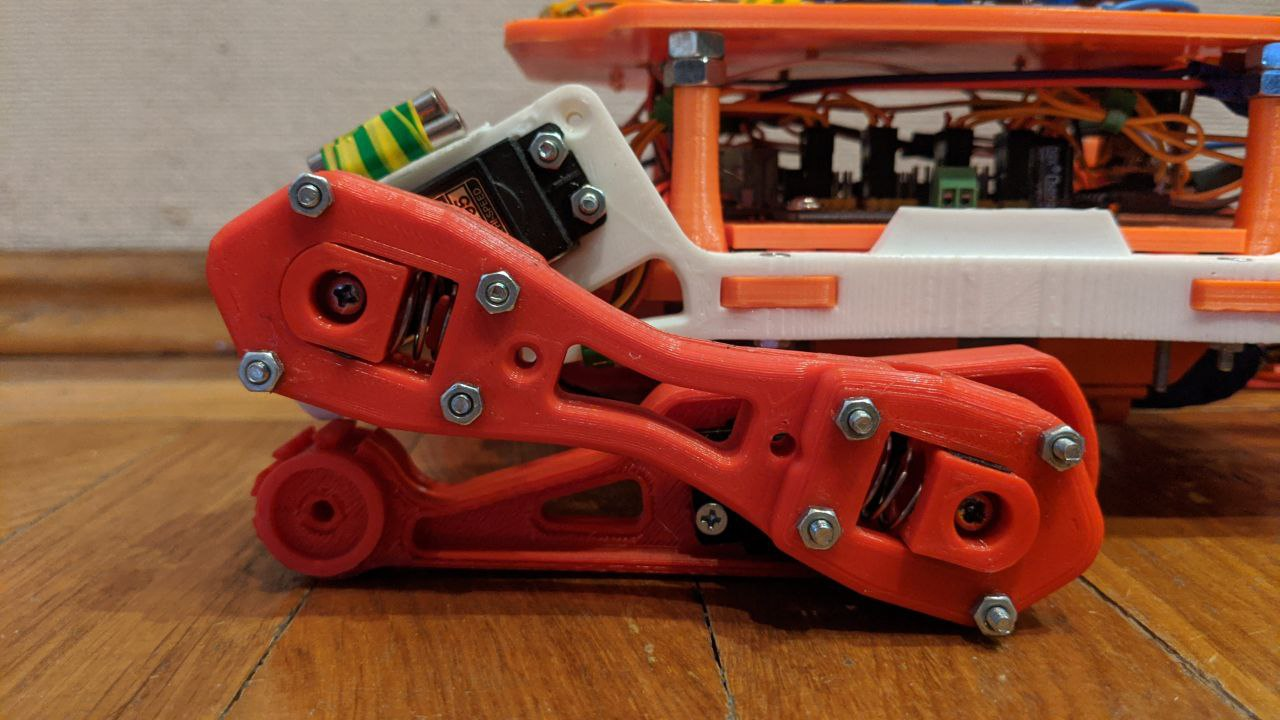
\includegraphics[width=0.5\textwidth]{leg3}
		\caption{Робот в исходном положении до инициализации.}
		\label{leg3}
	\end{center}
\end{figure}


\newpage
\section{Выбор серводвигателей.}\label{C4_3}


Сервопривод - это механический привод, который содержит датчик (для измерения положения, скорости, усилия и других параметров) и блок управления приводом (который может быть электронной схемой или механической системой тяг), что позволяет автоматически поддерживать необходимые параметры на датчике в соответствии с заданным внешним значением (например, положение ручки управления или численное значение от других систем). Сервопривод можно рассматривать как автоматического точного исполнителя, который получает на вход значение управляющего параметра в режиме реального времени и используя показания датчика, стремится создать и поддерживать это значение на выходе исполнительного элемента. В настоящей работе выбрана модель сервопривода MG995, основные характеристики которого сведены в таблице \ref{servoParam}.


\begin{table}[h]
	\begin{center}
		\caption{Характеристики сервопривода MG995}
		\label{servoParam}
		\begin{tabular}{| l | l |}
			\hline
			Общий вес   &    55 г \\ \hline
			Размеры (ШхВхГ) & 54х47.2х20 мм\\ \hline
			Крутящий момент & 8.5кгс/см (4.8В), 10кгс/см (6В) \\ \hline
			Рабочая скорость & 0.2с/60$^{\circ}$ (4.8В), 0.16с/60$^{\circ}$ (6В) \\ \hline
			Рабочее напряжение & 4.8В - 7.2В \\ \hline
			Рабочая температура & 0 C$^{\circ}$  - 55 C$^{\circ}$ \\ \hline
			Зона нечувствительности ШИМ & 5мкс \\ \hline
		\end{tabular}
	\end{center}
\end{table} 

Резкие изменения угла в серводвигателях являются следствием специфики их конструкции, а если быть точнее, то данная проблема связана с принципом работы потенциометра, который выполняет роль энкодера внутри двигателя. Таким образом принцип регулирования угла поворота состоит в подаче ШИМ сигнала посредством написанного программного обеспечения, сам сигнал преобразуется в напряжение благодаря работе потенциометра и приводит вал в заданное положение с максимальной скоростью. Из этого можно сделать вывод, что в используемых  сервоприводах не имеется обратной связи, и при использовании с тяжелыми объектами будут создаваться лишние нагрузки, которые будут приводить к потреблению тока, особенно это важно по отношению к стартовым токам. В нашем случае такое поведение потенциально приведет к уничтожению редуктора внутри двигателя (рисунок \ref{servo_scheme}), так как движимые объекты инерционные и такое управление для них неприемлемо. Эта проблема будет решаться также программно, а само решение описано в главе \ref (Глава 4 управление)  

%Резкие изменения угла в серводвигателях являются следствием специфической конструкции этих устройств. Более точно, данная проблема связана с принципом работы потенциометра, который выполняет роль энкодера внутри двигателя. Принцип регулирования угла поворота заключается в подаче ШИМ-сигнала через соответствующее программное обеспечение. Сам сигнал преобразуется в напряжение благодаря работе потенциометра, что позволяет валу быстро перемещаться в заданное положение. Отсутствие обратной связи в используемых сервоприводах может привести к нежелательному созданию лишних нагрузок при использовании с тяжелыми объектами, особенно это критично для стартовых токов. В нашем случае такое поведение потенциально способно привести к разрушению редуктора внутри двигателя (см. Рисунок \ref{servo_scheme}), поскольку управляемые объекты имеют инерционные характеристики, и этот тип управления неэффективен для них. Данная проблема также будет решаться с помощью программного обеспечения, и решение описано в главе \ref{}.

\begin{figure}[h!]
	\begin{center}
		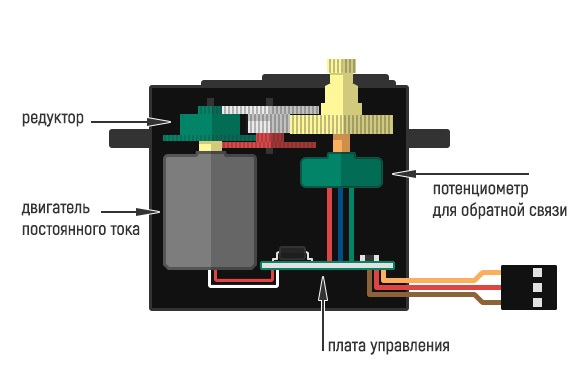
\includegraphics[width=0.7\textwidth]{servo_scheme}
		\caption{Схема сервопривода}
		\label{servo_scheme}
	\end{center}
\end{figure}

Еще одним последствием такого принципа работы выступает осложнение корректной сборки, так как для правильной конфигурации ноги на прототипе сервоприводам требуется калибровка. Иначе говоря, необходимо выставлять крайние положения ног и рассчитывать диапазон ШИМ сигнала и принимаемого угла, чтобы как можно точнее задавать положение ноги в будущем. Это достаточно неприятное следствие, так как каждая единица серводвигателя уникальна и требует отдельной калибровки. Методы калибровки в данной работе разбираться не будут.

\newpage